%TODO: refer to grid convolutions as discrete (?)


\chapter{Artificial Neural Networks}
\label{chap:neuralnetworks}

\textit{Feed forward artificial neural networks}, or less formally, \textit{neural networks}, are a class of machine learning algorithm which are loosely inspired by neuroscientific models of how biological neural networks operate\cite{mcculloch1943}. 
Like many machine learning methods, a neural network is a parameterized function with vector input and either scalar or vector output.
For example, the input may be pixel intensities from an image of interest, and the output may be an integer corresponding to a label which indicates the image's content.
In this thesis, the function is denoted $f(x|\Theta)$, where $x$ is the input vector and $\Theta$ is the complete set of parameters, or weights.
In neural networks, $f$ is composed of a sequence of layers, $h_i(x_i|\Theta_i)$ which perform comparatively simple mathematical operations on their input to produce a layer output.
By convention, the input vector is considered the first layer of a neural network, even though it performs no operations, and the output of the last layer is the output of the entire network.
All intermediate layers are termed \textit{hidden layers}, each of which accepts the output of the preceding layer and passes its output to the subsequent layer.
The number of layers in a neural network (besides the first layer) is its \textit{depth}, and the number of outputs of a given layer is the number of \textit{units} (or \textit{neurons}) in that layer.
Figure \ref{fig:twolayernetwork} depicts a two layer neural network with three inputs, four units in the hidden layer, and two outputs.

\begin{figure}
	\centering
	%\begin{center}
	\includegraphics[width=0.8\textwidth]{twolayernetwork.pdf}
	%\end{center}
	\caption{A two layer neural network with a single hidden layer.}
	\label{fig:twolayernetwork}
\end{figure}

A common form of hidden layer is a \textit{dense layer}, in which each unit calculates a weighted sum of the layer inputs, where the set of weights is unique to each unit.
It is also common to add a scalar bias term and apply a nonlinear activation function to the weighted sum.
Dense layers have a convenient mathematical representation:

\begin{equation}
h(x|W, b)=\sigma(W x^T + b),
\label{eq:denselayer}
\end{equation}

\noindent
where $W$ is a matrix of weights, $x$ is the layer input, $b$ is a vector of biases, and $\sigma(\cdot)$ is a nonlinear activation function.
If there are $n$ inputs to a layer and $m$ units in the layer, then $W\in\mathbb{R}^{nxm}$ and $b\in\mathbb{R}^{m}$.
The expression $W x^T + b$ is called the \textit{signal}, and $h$ the \textit{activation}.
For hidden layers, activations have traditionally taken the form of a sigmoidal, or "s-shaped", function such as the logistic function, $\sigma(x) = 1/(1+e^{-x})$, or hyperbolic tangent, $\sigma(x) = tanh(x)$.

Despite being conceptually simple, this formulation of artificial neural networks is capable of approximating any continuous function on a compact subset in $\mathbb{R}$ with arbitrarily small error~\cite{cybenko1989}.
The challenge of using neural networks for function approximation is in finding the appropriate set of parameters to approximate the desired function.
For simple feed forward neural networks, this is accomplished by quantifying the error between the desired function and the approximation for a given training data set $X=(x_1, x_2, ..., x_N)$, using a differentiable loss function $L(\Theta | X)$. 
The weights are updated by differentiating $L$ with respect to $\Theta$ and "taking a step" in parameter space opposite the direction of the gradient. 
This update step can be repeated iteratively in a process called \textit{gradient descent}, which can be dated back to Augustin-Louis Cauchy~\cite{cauchy1847}.
Mathematically, 
\begin{equation}
\Theta_{k+1} = \Theta_k - \eta \nabla L(\Theta_k | X) = \Theta_k - \eta \sum_{n=1}^{N} \nabla L(\Theta_k | x_n),
\label{eq:batch_gd}
\end{equation}

\noindent
where $\eta$ is a tunable step size and $k$ indicates the iteration.
The gradient can be efficiently calculated using automatic differentiation~\cite{linnainmaa1976}, in which the update step is referred to as \textit{backpropagation}.
Weights are usually initialized by drawing from distributions that have some empirical or theoretical justification~\cite{glorot2010}.
A variant of this algorithm, called stochastic gradient descent (SCG) performs an update using a gradient computed from a random sample of the training data at each iteration.
There is also a batched version where the training data are randomly shuffled and divided into a fixed number of equal sized \textit{mini-batches} and an update is performed on each one. 
When all mini-batches have been used in an update step, this constitutes an \textit{epoch}.
Gradient descent is a first order method, however various second order methods have also been used to train neural networks~\cite{fletcher1964, polak1969, moller1993, marquardt1963}.

Like many machine learning algorithms, neural networks risk \textit{overfitting}, in which the network learns to approximate the training data (which usually contain noise), rather than the underlying function from which the training data are assumed to be drawn.
This hinders the ability of neural networks to generalize to unseen data.
In neural networks, overfitting is commonly the result of an overcomplete parameterization coupled with overtraining~\cite{reed1993, dalianis1993}.
Many regularization techniques have been introduced to prevent overfitting of neural networks, including early stopping~\cite{morgan1990}, model pruning~\cite{reed1993}, weight decay\cite{krogh1992}, lateral inhibition~\cite{krizhevsky2012}, induced sparsity~\cite{ng2011, makhzani2015}, and dropout~\cite{srivastava2014}, with dropout being one of the most common. 
Dropout consists of randomly dropping units from the neural network during the training phase.
Each time a training example is presented to the network, each unit in the network is dropped with probability $p$, commonly 0.5.
Each application of dropout can be seen as generating a new network whose units are a subset of the units in the original network.
Given $n$ units in a network, there are $2^n$ possible dropout networks all with a high degree of weight sharing.
During testing, no dropout is performed, and weights are rescaling by $p$.
This has the effect of averaging the prediction of each dropout network.
Dropout helps prevent overfitting by limiting the effective number of parameters in each dropout network and reducing the amount of co-adaptation among units in the network.\cite{srivastava2014}.


In recent years, more advanced forms of neural networks under the moniker \textit{deep learning} have demonstrated success in sophisticated tasks, particularly for image and speech recognition~\cite{krizhevsky2012, lecun2015, masci2011, hinton2012, he2016}, but also in a variety of other applications such as quantitative structure activity relationship (QSAR) prediction~\cite{ma2015}, particle detection~\cite{ciodaro2012}, and reinforcement learning\cite{mnih2015}.
These advances were catalyzed by the availability of large volumes of labeled data\cite{deng2009, krizhevsky2009} and the improvements in computing power from general purpose graphical processing units (GP-GPUs) and distributed systems\cite{chetlur2014, chu2007}.
Such factors allow experimentation with larger networks and more complicated layer operations such as convolutions, which are described in the following section.

\section{Convolutional Neural Networks}

Accurately labeling an image using a neural network often relies on the network's ability to detect low level features in the image such as edges and textures, which collectively indicate the content of an image~\cite{ng2011}.
This is accomplished through the appropriate set of parameters, which maximize a unit's activation when presented with a feature of interest.
These parameters can be learned through the standard backpropagation algorithm using training images. 
The challenge, however, is that the training data may not present the features of interest in all regions of the input. 
For example, suppose the labeling task is to determine if an image does or does not contain a cat.
Suppose further that no training image contains a cat in the upper left corner of the image.
Therefore it is possible, even if the network has learned which low level features indicate the presence of a cat, that it will not recognize a cat contained in the upper left corner of the image, since it has not been explicitly shown examples of this.
This may seem unlikely, but consider that the network does not incorporate any semantic meaning of the word "cat", only that a certain set of example images are positive examples and a certain set are negative examples.
Indeed, consider the slightly different labeling task where the classes being considered are "contains a cat anywhere but the top left corner" and its negation.
In this case, the same set of training images are appropriate and the hope is that the network would \textit{not} classify images with cats in the upper left corner as positive examples.
In most cases, the labeling task is more like the former example than the latter, in which case it would be beneficial for the network to learn to detect objects in a \textit{translation invariant} fashion. 
This is the primary purpose of convolutional layers.

The term convolution is inherited from field of functional analysis, where two functions, $f$ and $g$, are combined in the following way to generate a third function, $(f*g)$:

\begin{equation}
(f*g)(t) = \int_{-\infty}^{\infty}f(\tau)~g(t-\tau)~d\tau
\label{eq:math_conv}
\end{equation}

\noindent
The convolution can be interpreted as reversing one function, shifting it with respect to the other function, and integrating the product. 
Each value of $t$ represents a different relative shift.
The discrete analog of this, assuming a regular domain, takes the sum of the elementwise product of two infinite arrays.
This can be extended to two dimensions by taking the sum of the elementwise product of two matrices.
Finite matrices can be considered by reinterpreting the matrices as infinite and zero everywhere outside a region the same size as the finite matrix.
%TODO: Figure of grid?
This discrete, two dimensional, and finite analog to convolution forms the basis of convolutional layers in neural networks.

Consider a monochrome image as a finite matrix where the matrix entries reflect pixel values in the image. 
Further, consider a smaller matrix called a filter where the matrix entries are filter weights.
By convolving the filter over the input image, a new matrix is created where each value is the result of summing the elementwise product of the image and filter with the filter in a particular position.
Figure \ref{fig:convolutionallayer} depicts the application of a filter to the input in a particular image.
The elementwise product naturally extends to images with multiple \textit{channels} (colors) as long as the filter has the same number of channels as the image.
The result of a convolution in a particular position depends on the values of the input image and the weights, and indeed there exist weights which produce larger outputs only in the presence of particular local features in the input.
Hence convolutions can be used in a neural network to detect patterns in the input.
Furthermore, since the same set of weights is used to convolve across the whole image, feature detection can be performed in a translation invariant way as desired. 
A filter may only detect a particular local feature, so multiple filters can be used to detect multiple features simultaneously, each producing a different channel in the output.
Note that the output of a convolution layer resembles the structure of the input, so convolutional layers may be stacked.


\begin{figure}
	\centering
	%\begin{center}
	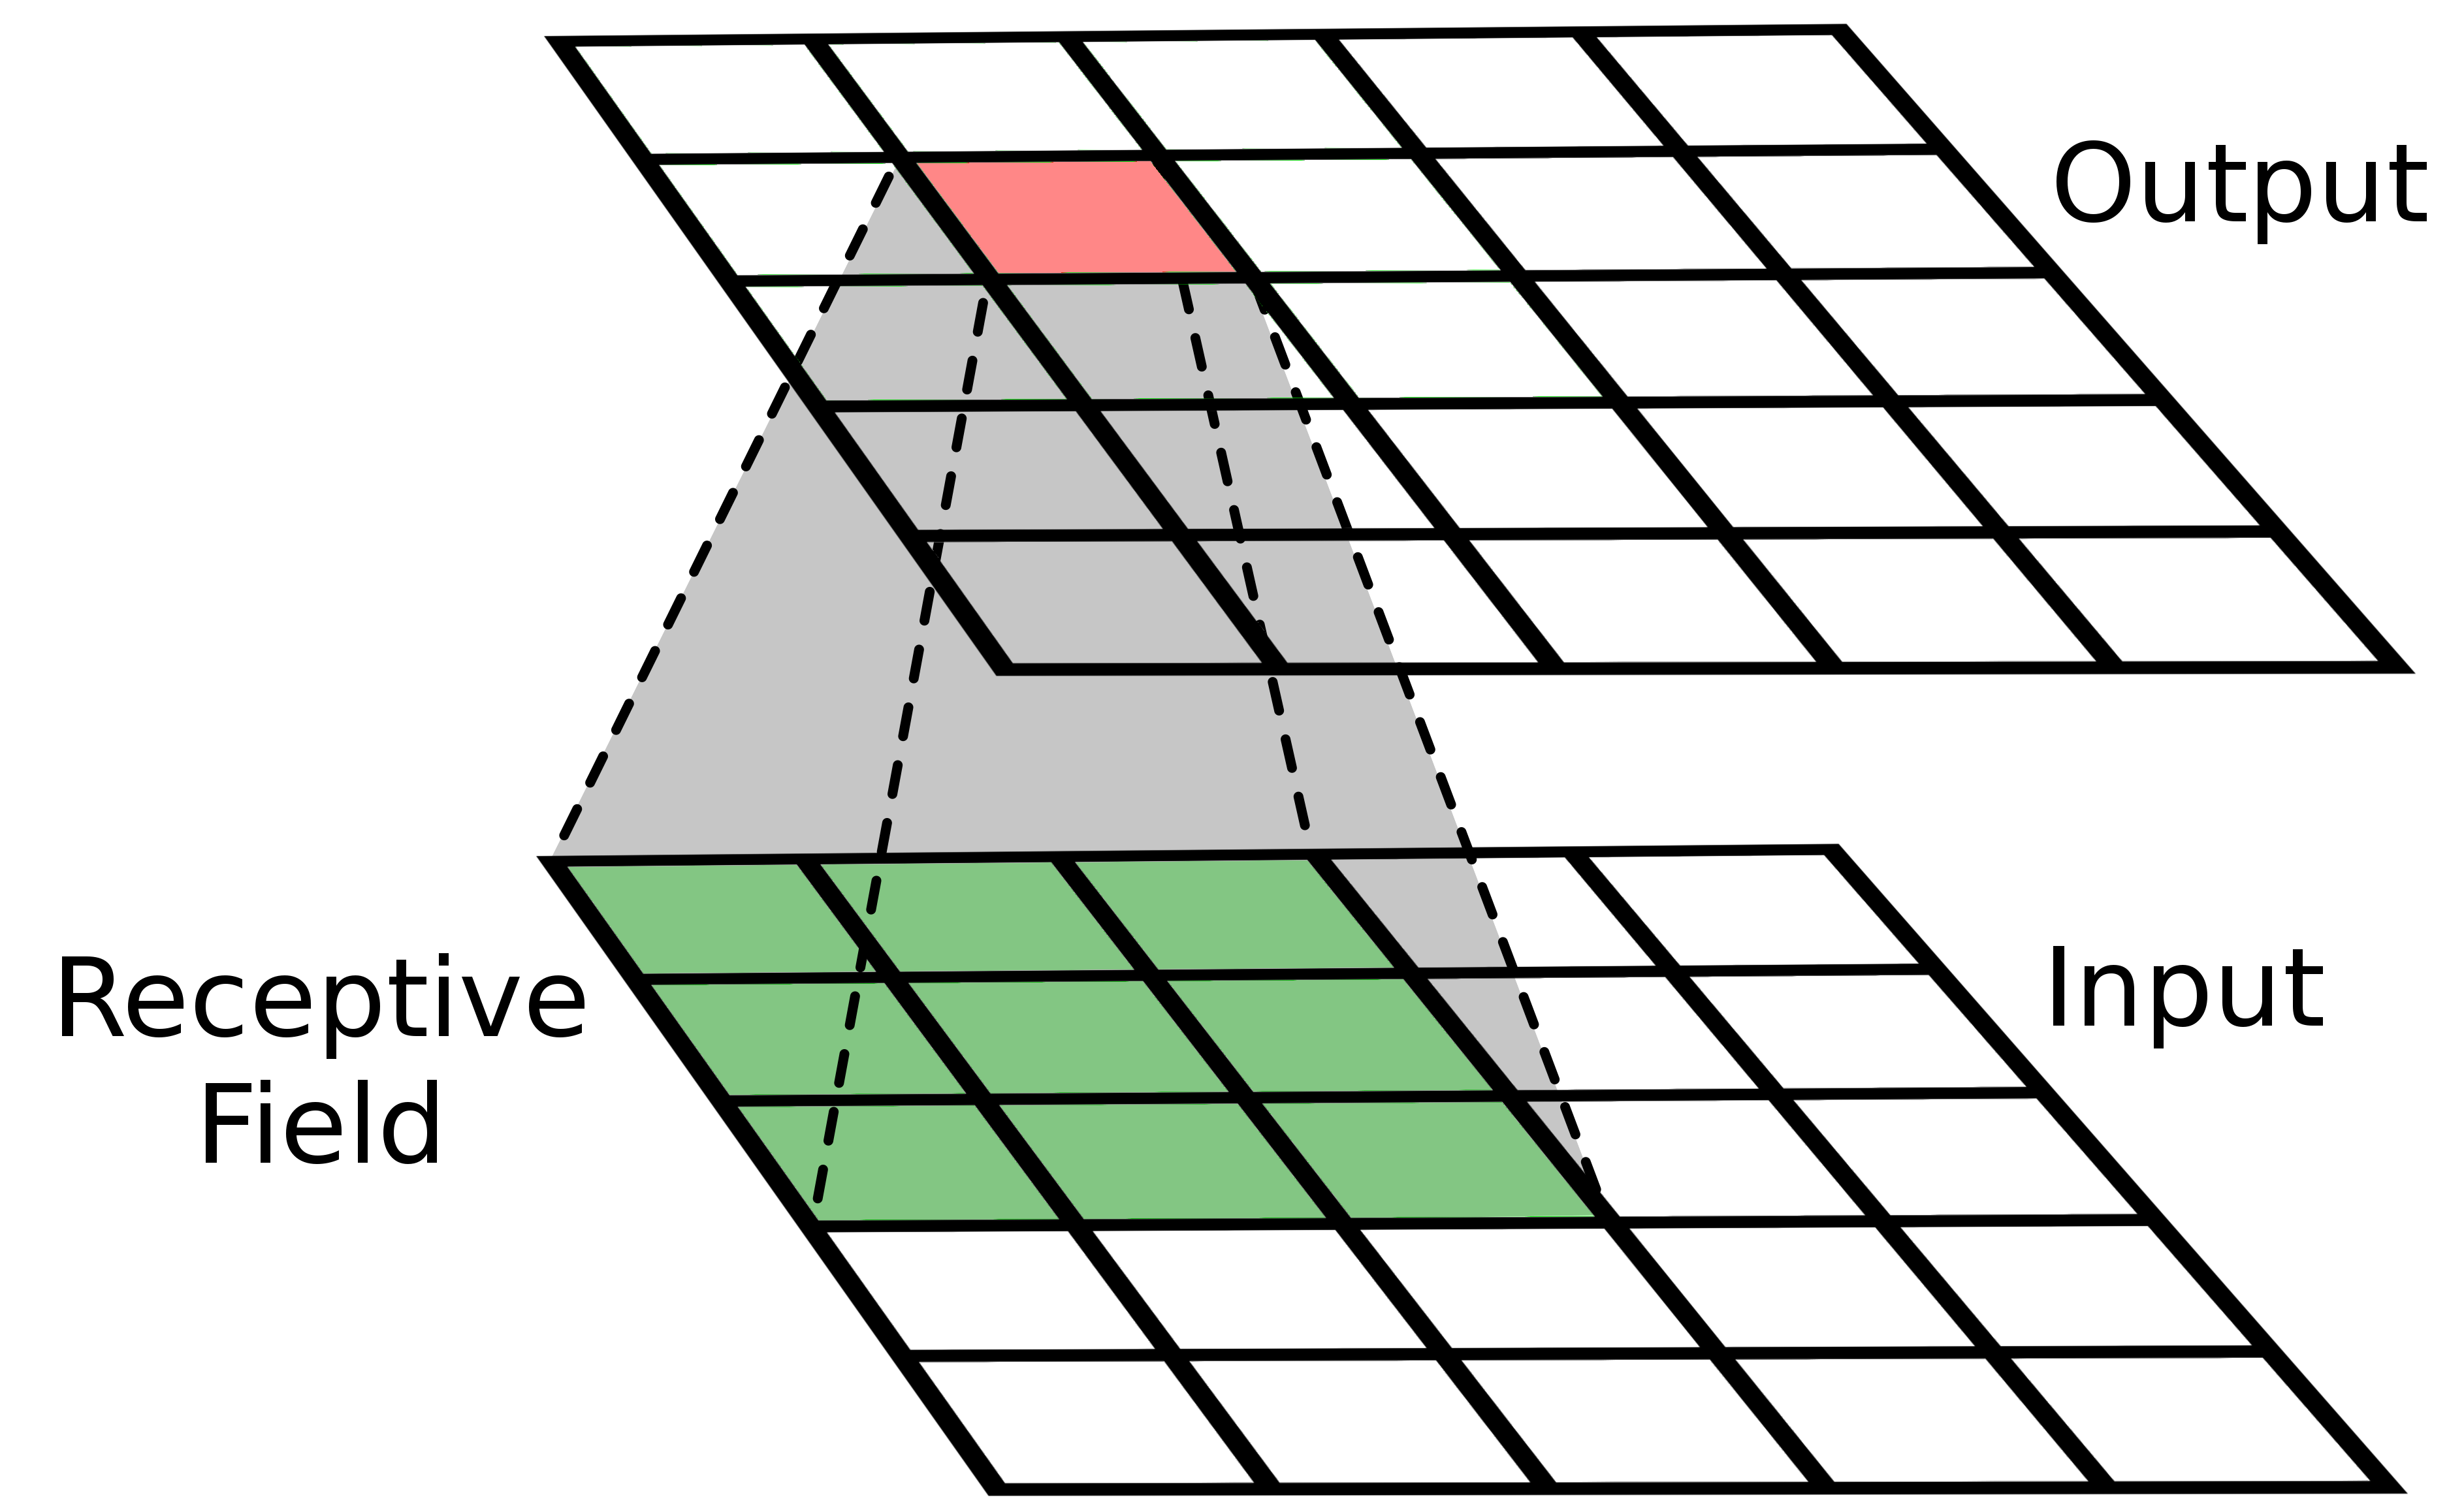
\includegraphics[width=0.8\textwidth]{conv_grid.png}
	%\end{center}
	\caption{Application of a 3x3 convolution filter to an input grid. The filter is multiplied elementwise with the receptive field (in green) and produces a scalar output (in red).}
	\label{fig:convolutionallayer}
\end{figure}

The design of convolutional layers gives rise to certain properties which prove useful in image related tasks:
 \begin{itemize}
 	\item \textit{Structural awareness}
 	Convolutional filters are constructed so that they exploit the structural characteristics of the input.
 	Rather than treat each pixel of an image as independent of all others, convolutions operate on local regions of pixels, allowing filters to detect spatial correlations in a straightforward manner.
 	\item \textit{Locality}. 
 	Filters are typically significantly smaller than the size of the input, so a given position they are operating on a local neighborhood (also called a \textit{receptive field}) of the input image. 
 	Any features learned by a filter will necessarily be local as well. 
 	The advantage of local features is that they are simpler and more universal than more global features, so that filters which detect edges or textures will be more useful to subsequent layers in the network than a filter which recognizes a specific object or animal, for example. 
 	One exception to locality is when layers are stacked on top of one another, resulting a larger "effective" receptive field on the original input for filters later in the network.
 	This exception is actually advantageous for abstraction (see below).
 	\item \textit{Translation invariance}. 
 	As discussed, a filter "inspects" each part of the image for a particular pattern, regardless of where that pattern occurred in the training images.
 	This improves generalizability because during training certain features may be presented in limited regions of the image, but detection of that feature can still operate on a global scale.
 	\item \textit{Abstraction}. Whereas a network's first convolutional layer detects patterns in the input, subsequent layers detect patterns in the output of previous layers. 
 	This promotes a hierarchical abstraction of the input, where early layers detect local features, and subsequent layers combine features into more complex objects. 
 	For example, early filters may detect edges of varying orientations, middle filters may detect combinations of edges which indicate curves in space, and latter filters may detect combinations of curves which indicate a particular handwritten letter or digit.
 	\item \textit{Resistence to overfitting}. 
 	One interpretation of a convolutional layer is that each filter is a series of units, each responsible for a distinct receptive field on the input.
 	A unit has nonzero weights only for the regions of the input in its receptive field, and all units share the same weights. 
 	This combination of weight sharing and sparsity make a convolutional layer less prone to overfitting compared to a dense layer with the same number of units.
 \end{itemize}

Convolutional neural networks often incorporate \textit{pooling layers}, which reduce a small region of the input (e.g. 2x2 pixels for an image) to a single grid element that takes either the maximum or average value (per channel) of the region. 
Pooling allows downsampling of the grid, and is often performed between convolutional layers. 
It's also common to include a series of dense layers after all convolutional layers which essentially combine the results of convolution in a way relevant to the learning task.
Because the number of parameters in convolutional layers, the final dense layers often contain the majority of the parameters in the network.


 The above properties make convolutional layers well suited for structured data with a natural hierarchy of abstraction.
 The primary-secondary-tertiary-quaternary structural hierarchy of proteins suggests that they fulfill the first requirement.
 Unfortunately, neither protein residues, nor their constituent atoms are aligned in a regular grid, so the above definition of convolution cannot be directly applied. 
 In the Chapter \ref{chap:methods}, new convolutions are introduced which operate on irregular structures, namely graphs, and a graphical model of proteins is presented which allows use of these graph convolutions for protein interface prediction. 